\chapter{Einleitung}

\section{Motivation}
\"Ublicherweise nehmen \"Uberwachungssysteme den betreffenden Bereich von 24 Stunden am Tag auf. Das erzeugt eine Menge \"Uberwachungsmaterial, in dem man schnell die \"Ubersicht verliert und unn\"otig viel Speicherkapazit\"at verbraucht.\\
\\
Wenn eine kontinuierliche Aufzeichnung eines Bereichs nicht erforderlich ist, kann der \"Uberwachungsprozess durch "on-demand"-Betrieb der Anlage optimiert werden. 
Die Grundidee hinder dem Projekt ist, einen Geb\"aude-Zugang nur dann aktiv zu \"uberwachen, wenn er genutzt wird (i.e. wenn die T\"ur ge\"offnet wird).
\\

\section{Ziele}
Erstellt werden soll ein System zur automatischen Eintritts\"uberwachung an Geb\"aude-Zug\"angen.\\
\\
Das System soll vollst\"andig autonom Video-Aufnahmen von Personen machen, welche den vom System \"uberwachten Zugang nutzen.
Zu diesem Zweck wird ein Raspberry Pi mit Kamera und Magnetschalter ausgestattet. \\
\\
Der Magnetschalter wird an der T\"ur des zu \"uberwachenden Zugangs positioniert, sodass  er \"offnet/schlie{\ss}t, wenn die T\"ur ge\"offnet/geschlossen wird.
Die Kamera wird mit Blickrichtung zur T\"ur positioniert, um sp\"ater im Video das Gesicht der Person erkennen zu k\"onnen.\\
\\
Sobald nun der Magnetschalter das \"Offnen der T\"ur meldet, beginnt die Aufzeichnung des \"Uberwachungs-Videos \"uber die Kamera. Die Aufzeichnung wird fortgesetzt soange die T\"ur offen bleibt. Wird die T\"ur geschlossen, wird die Aufnahme nach einigen Sekunden beendet.\\
Durch die Verz\"ogerung des Aufnahme-Stopps soll sichergestellt werden, dass im Fall einer Manipulation des Magnetschalters (z.B. mit K\"uhlschrank-Magnet) immer noch ausreichend \"Uberwachungsmaterial gesammelt wird.\\
\\
Alle Aktivit\"aten werden mit Zeitstempel und Verweis auf die Video-Dateien in der Datenbank des Raspberry Pi hinterlegt.
\"Uber ein im lokalen Netz erreichbares Webinterface k\"onnen Zugangszeiten und die damit assoziierten Aufzeichnungen eingesehen/heruntergeladen werden.\\
Videomaterial \"alter als der konfigurierte Zeitraum wird gel\"oscht.\\
\\
Das System ist nicht als Alarmanlage oder Schutzma{\ss}nahme gegen Einbruch zu verstehen.
\\

\section{Eigene Leistung}
Die eigene Leistung umfasst neben der schriftlichen Ausarbeitung die Erstellung eines Prototyps mithilfe der ausgew\"ahlten Hardware und Software als Beweis f\"ur die Realiserbarkeit der Projektidee.

\newpage

\section{Gantt-Diagramm}

\begin{figure}[ht]
    \centering
    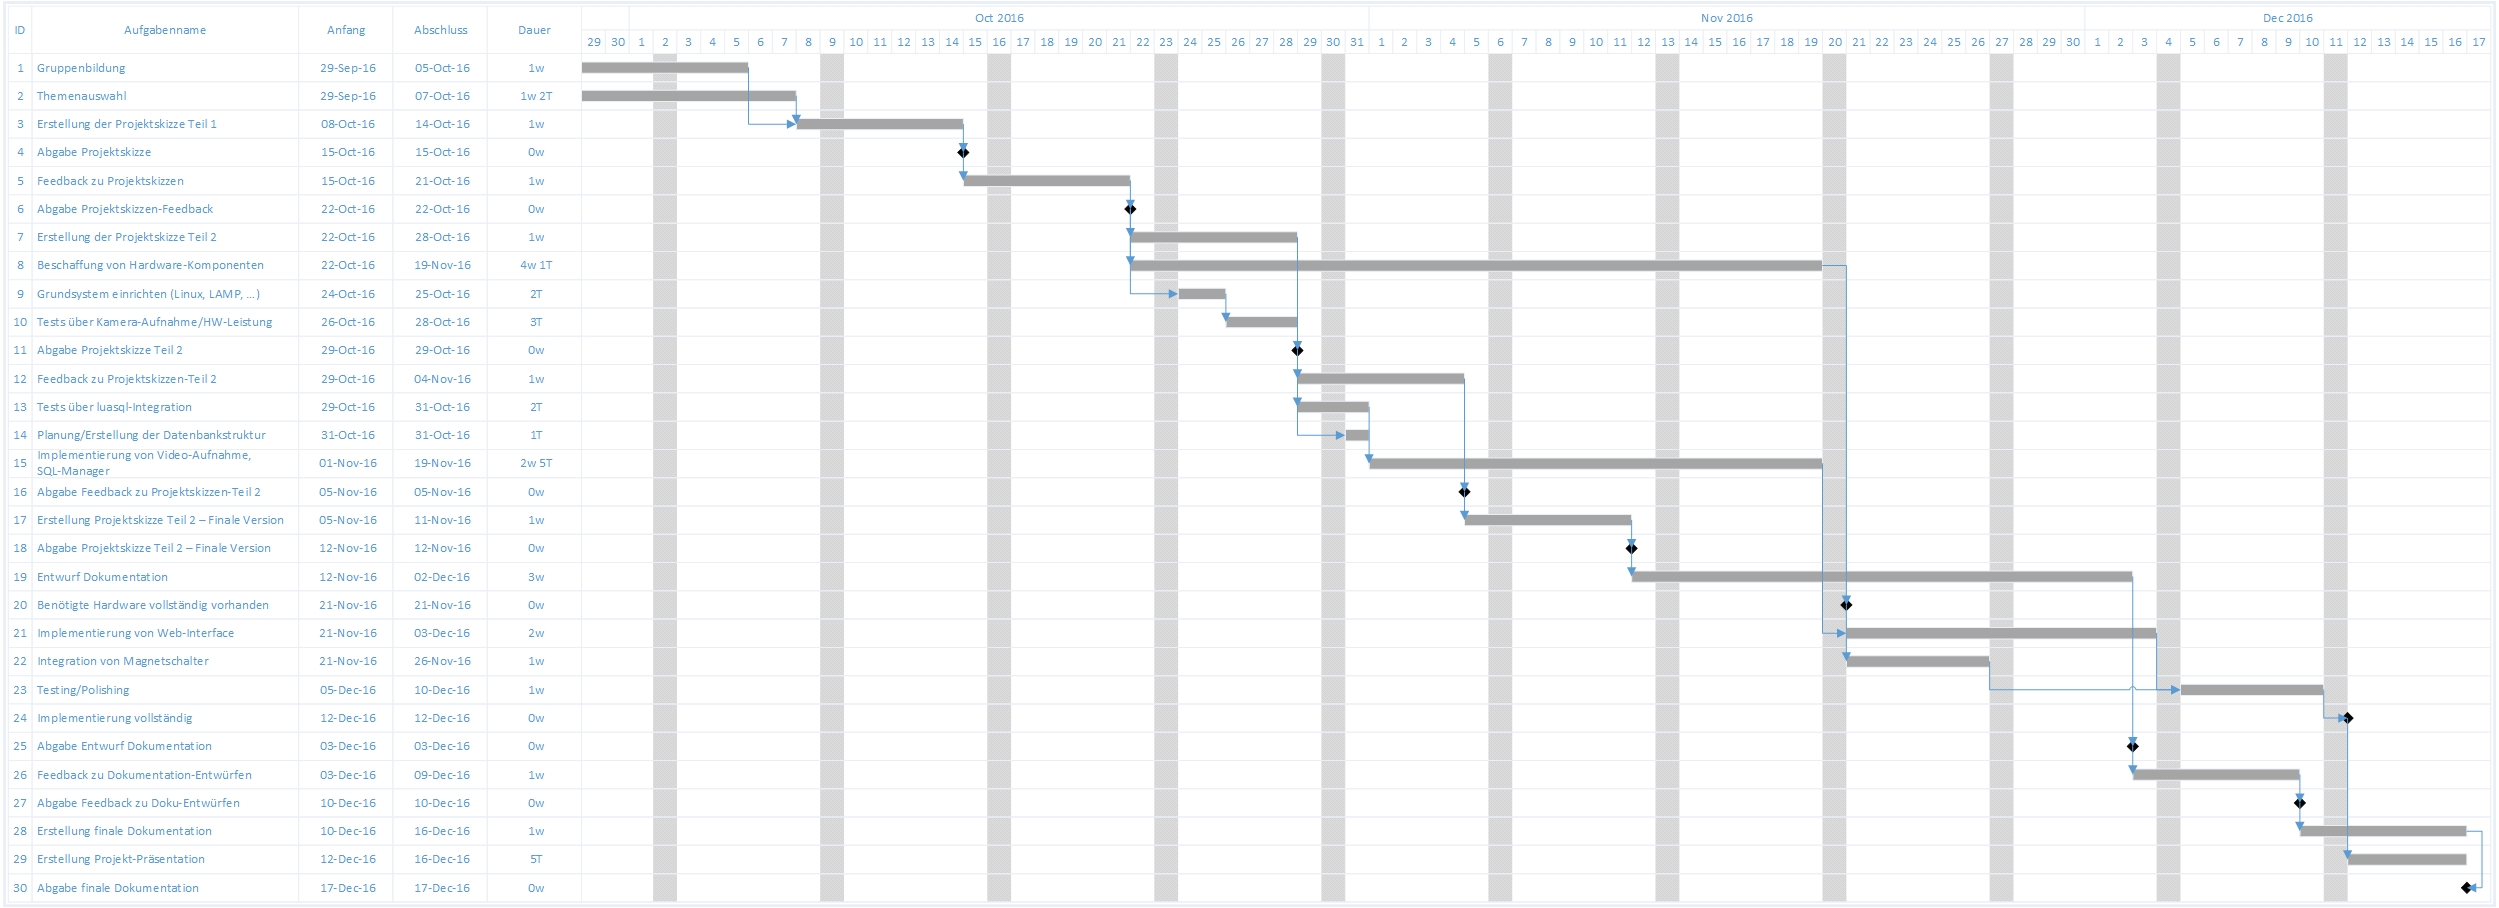
\includegraphics[angle=90,scale=0.3]{images/gantt}
    %\caption{Gantt-Diagramm}
    \label{fig:gantt}
\end{figure}

\newpage